\chapter{الخلط، والتذبذب، وعزوم ثنائية القطب الكهربائية، ومؤثرات الحقول}

نبدأ خارج الموضوع المعلن قليلًا، بسؤال عن النيوترينوات. توجد أدلة على أن للنيوترينوات كتلة، وأن أنواع النيوترينو تختلط. فإذا لم تكن الكتل كلها متساوية، فكيف يمكن لنوعٍ أن يتحول إلى آخر من دون انتهاك حفظ الطاقة؟

يشير هذا السؤال إلى نمط يظهر في ميكانيكا الكم كلها: فالحالات التي يُحضَّر فيها نظام أو يُكشَف فيها عنه ليست بالضرورة الحالات التي تجعل هاملتونيه قطريًا. والحالة ذات الطاقة المحددة لا تكتسب إلا طورًا. أما الحالة المُحضَّرة التي هي تراكب لعدة طاقات فتتغير لأن مركباتها تكتسب أطوارًا مختلفة. وسيحملنا هذا التمييز من بئر مزدوج إلى تذبذب النيوترينو وسبق السبين. وبعد استطراد عن عزم ثنائي القطب الكهربائي للإلكترون، سنعود إلى التكميم الثاني ونرى البنية الفورييهية نفسها للموضع--الزخم على مستوى المؤثرات.

\section{الخلط بوصفه القضية الحقيقية}

لا يلزم أن تكون جميع النيوترينوات ذات الكتلة نفسها. فالحالات الذاتية للطاقة لا تختلط بعضها ببعض؛ إذ يتطور كلٌّ منها على نحو مستقل. وما نسميه \emph{النوع}، أو النكهة، في النيوترينو يرتبط بكيفية إنتاجه وكشفه، ويمكن لحالة النكهة أن تكون تركيبًا خطيًا من الحالات الذاتية للكتلة والطاقة. وعلى نحو تخطيطي،
\begin{equation}
|\text{type}\rangle = \sum_n c_n |E_n\rangle .
\end{equation}
ومن ثم فالصياغة الصحيحة ليست أن الحالات الذاتية للطاقة تتحول بعضها إلى بعض، بل إن الحالات المسماة ``نيوترينو إلكتروني'' أو ``نيوترينو ميوني'' ليست بالضرورة، في حد ذاتها، حالاتٍ ذاتية للطاقة.

\begin{classroomqa}
\lecturetimestamp{00:00:09}
\audiencequestion{إذا كانت للنيوترينوات كتل مختلفة، فكيف يمكنها أن تختلط مع بقاء الطاقة محفوظة؟}
\lecturerresponse{الحالات الذاتية للكتلة والطاقة لا تتحول بعضها إلى بعض. وحالات نكهة الإلكترون والميون والتاو هي تراكيب خطية مختلفة من تلك الحالات الذاتية. ويتطور كل مركِّب كتلي بطوره الخاص، ويغيِّر التداخل احتمالات النكهة من غير انتهاك حفظ الطاقة.}
\end{classroomqa}

لهذه البنية أمثلة كثيرة. وأوضحها يبدأ بجسيم في بئر مزدوج متناظر.

\section{البئر المزدوج المتناظر والحالات المتموضعة التقريبية}

لننظر إلى جسيم يتحرك في كمون بئر مزدوج متناظر، بين القاعين فيه حاجز عالٍ. فإذا اعتُبر الحاجز لا نهائي الارتفاع، انفصلت البئران اليسرى واليمنى انفصالًا تامًا. وعندئذ يمكن حل البئر اليسرى كما لو أن البئر اليمنى غير موجودة، وبالمثل للبئر اليمنى. وتكون دالتا الموجة التقريبيتان للحالة القاعية عندئذ حالةً متموضعة إلى اليسار \(\psi_L\) وحالةً متموضعة إلى اليمين \(\psi_R\)، وكلتاهما بالطاقة نفسها \(E\).

في كل بئر معزول تمتلك الحالة القاعية الخواص النوعية المألوفة: فهي ملساء، ولا تحوي عقدًا، وتقع عند أخفض طاقة ممكنة تتسق مع الاحتجاز. تخيل الحاجز المركزي العالي جدارًا من الطوب. إن التعامل معه على أنه لا نهائي ليس إلا تقريبًا، لكنه يزوِّدنا بزوج مفيد من الحالات المتموضعة نبدأ منه.

\begin{figure}
\centering
\begin{adjustbox}{max width=\linewidth}
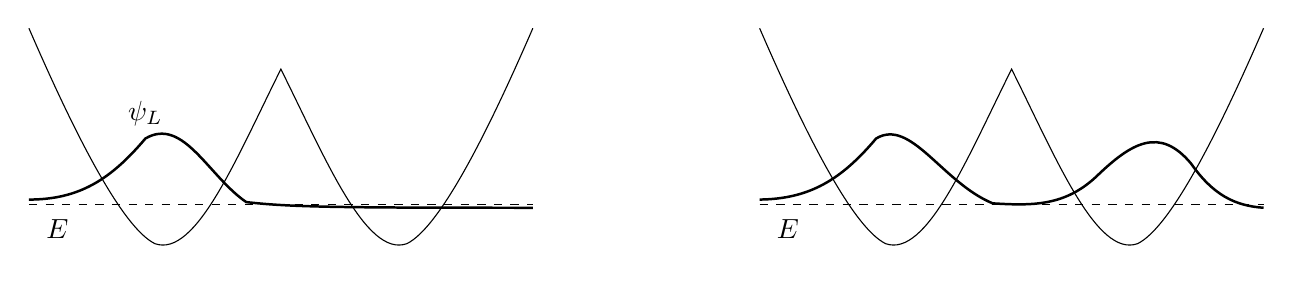
\begin{tikzpicture}[x=0.8cm,y=0.8cm]
\begin{scope}[shift={(-5.8,0)}]
\draw (-4,2.7) .. controls (-3.35,1.2) and (-2.55,-0.45) .. (-2.0,-0.72)
      .. controls (-1.35,-0.95) and (-0.7,0.65) .. (0,2.05)
      .. controls (0.7,0.65) and (1.35,-0.95) .. (2.0,-0.72)
      .. controls (2.55,-0.45) and (3.35,1.2) .. (4,2.7);
\draw[dashed] (-4,-0.10) -- (4,-0.10);
\node at (-3.55,-0.48) {$E$};
\draw[line width=0.9pt] (-4,-0.02) .. controls (-3.2,-0.02) and (-2.7,0.30) .. (-2.15,0.95)
      .. controls (-1.55,1.30) and (-1.15,0.35) .. (-0.55,-0.06)
      .. controls (0.15,-0.14) and (0.9,-0.15) .. (4,-0.15);
\node at (-2.15,1.35) {$\psi_L$};
\end{scope}
\begin{scope}[shift={(5.8,0)}]
\draw (-4,2.7) .. controls (-3.35,1.2) and (-2.55,-0.45) .. (-2.0,-0.72)
      .. controls (-1.35,-0.95) and (-0.7,0.65) .. (0,2.05)
      .. controls (0.7,0.65) and (1.35,-0.95) .. (2.0,-0.72)
      .. controls (2.55,-0.45) and (3.35,1.2) .. (4,2.7);
\draw[dashed] (-4,-0.10) -- (4,-0.10);
\node at (-3.55,-0.48) {$E$};
\draw[line width=0.9pt] (-4,-0.02) .. controls (-3.2,-0.01) and (-2.7,0.30) .. (-2.15,0.95)
      .. controls (-1.6,1.28) and (-1.1,0.25) .. (-0.30,-0.08)
      .. controls (0.35,-0.12) and (0.85,-0.12) .. (1.35,0.35)
      .. controls (1.9,0.88) and (2.35,1.15) .. (2.85,0.55)
      .. controls (3.2,0.05) and (3.55,-0.12) .. (4,-0.15);
\end{scope}
\end{tikzpicture}
\end{adjustbox}
\caption{إعادة رسم نظيفة لرسومات اللوح الافتتاحية. على اليسار توجد الحالة التجريبية أحادية الجانب \(\psi_L\)، الناتجة عن افتراض أن الحاجز لا نهائي فعليًا. وعلى اليمين مُدَّت دالة الموجة نفسها على نحو متناظر عبر الحاجز، موضحةً التسرب الصغير لكنه غير المنعدم الذي يُنتج في النهاية الحالة القاعية الزوجية الحقيقية.}
\end{figure}

لكن الحاجز، من منظور ميكانيكا الكم، ليس لا نهائيًا حقًا. فدالة الموجة في منطقة الحاجز ليست صفرًا تمامًا؛ إنها صغيرة جدًا فحسب. وهذا التسرب الضئيل هو القصة كلها. وهو ما يحول تقريب اليسار واليمين إلى مسألة خلط حقيقية.

\section{الحالات الذاتية للتكافؤ وانشطار المستويات الأسي}

تنقطع الآن الصورة المتموضعة بنظرية: إذا كان الكمون متناظرًا، أمكن اختيار الدوال الذاتية الدقيقة للطاقة بحيث تكون إما متناظرة أو متضادة التناظر تحت الانعكاس.

\begin{theorem}
إذا كان \(V(x)=V(-x)\) في بعدٍ واحد، أمكن اختيار الدوال الذاتية للهاملتوني بحيث تحقق إما
\[
\psi(x)=\psi(-x)
\qquad \text{or} \qquad
\psi(x)=-\psi(-x).
\]
\end{theorem}

الآن يأتي التصحيح. فالحالتان أحاديتا الجانب \(\psi_L\) و\(\psi_R\) ليستا متناظرتين ولا متضادتي التناظر، ولذلك لا يمكن أن تكونا حالتين ذاتيتين دقيقتين للهاملتوني الكامل. وهما حالتان تقريبيتان جيدتان فقط عندما يكون الحاجز عاليًا. أما الحالات الذاتية الحقيقية فهي التركيبان المتناظر والمتضاد التناظر،
\begin{align}
\psi_+ &= \frac{\psi_L+\psi_R}{\sqrt{2}},\\
\psi_- &= \frac{\psi_L-\psi_R}{\sqrt{2}}.
\end{align}
وباستخدام الترميز الذي سيبقى على اللوح، نرمز إلى طاقتيهما بـ
\begin{align}
H\psi_+ &= (E_1-\epsilon)\psi_+,\\
H\psi_- &= (E_1+\epsilon)\psi_-.
\end{align}
ومن ثم يكون الانشطار الكلي
\begin{equation}
\Delta E = (E_1+\epsilon)-(E_1-\epsilon)=2\epsilon .
\end{equation}

\begin{figure}[htbp]
\centering
\includegraphics[width=0.92\linewidth]{lecture_08_frame_02.png}
\caption{دالة الموجة الممدودة تناظريًا في كمون البئر المزدوج. سعتها صغيرة لكنها غير منعدمة تحت الحاجز، وهذا هو أصل انشطار المستويات.}
\lectureframe{00:06:19}
\end{figure}

\begin{figure}
\centering
\begin{tikzpicture}[x=1cm,y=1cm]
\draw[->] (0,0) -- (0,3);
\node[left] at (0,2.8) {energy};
\draw (-0.35,1.60) -- (0.35,1.60);
\node[left] at (-0.45,1.60) {$\psi_L,\psi_R$};
\node at (1.7,1.60) {$\Longrightarrow$};
\draw (3.0,1.32) -- (3.75,1.32);
\draw (3.0,1.88) -- (3.75,1.88);
\draw[dashed] (2.8,1.60) -- (3.95,1.60);
\node[right] at (3.9,1.32) {$\psi_+,\ E_1-\epsilon$};
\node[right] at (3.9,1.88) {$\psi_-,\ E_1+\epsilon$};
\node[below] at (3.37,1.60) {$E_1$};
\end{tikzpicture}
\caption{منطق انشطار النفق كما على اللوح. حالتا اليسار واليمين التقريبيتان متكافئتان تقريبًا في الطاقة، لكن الحالتين الذاتيتين الدقيقتين المتناظرة والمتضادة التناظر تفصل بينهما قيمة صغيرة \(2\epsilon\).}
\end{figure}

يحمل ترتيب المستويات المغزى الفيزيائي. فالحالة المتناظرة أخفض قليلًا في الطاقة لأنها أكثر نعومة عبر منطقة الحاجز؛ والسماح لدالة الموجة بأن تتسرب وتستمر تناظريًا يخفض الطاقة بمقدار ضئيل جدًا. أما الحالة المتضادة التناظر فهي أعلى قليلًا لأن أول حالة مثارة في بعد واحد لها عقدة واحدة، وفي هذه المسألة المتناظرة تقع تلك العقدة عند المنتصف. والانحناء الإضافي يكلّف طاقة حركية.

الأثر صغير جدًا، بل صغير أسيًا في عرض الحاجز وارتفاعه. لسنا بحاجة هنا إلى صيغة WKB صريحة؛ فالنقطة المهمة هي أن الانشطار حقيقي ولكنه ضئيل. وتذكَّر أيضًا أن الإشارة الكلية لدالة الموجة لا تحمل أي معلومات فيزيائية. إن استبدال \(\psi_-\) بـ \(-\psi_-\) لا يغير الحالة.

\section{التطور الزمني وتذبذب اليسار واليمين}

لنطرح الآن السؤال الديناميكي: ماذا يحدث إذا وضعنا جسيمًا في البئر اليسرى؟ هذه هي الخطوة الحاسمة، لأن التذبذب هو الوجه المعتمد على الزمن لظاهرة الخلط نفسها.

العلاقات العكسية هي
\begin{align}
\psi_L &= \frac{\psi_+ + \psi_-}{\sqrt{2}},\\
\psi_R &= \frac{\psi_+ - \psi_-}{\sqrt{2}}.
\end{align}
ومن ثم فإن الحالة المتموضعة ابتداءً إلى اليسار هي
\begin{equation}
\psi(0)=\psi_L=\frac{\psi_+ + \psi_-}{\sqrt{2}}.
\end{equation}
وهذه ليست حالةً ذاتية للطاقة، ولذلك لا بد أن تتطور على نحو غير تافه.

نستخدم اصطلاح Schr\"odinger القياسي \(e^{-iEt}\). فالطور المشترك لا أثر ملحوظًا له؛ وإنما الطور النسبي بين مركبتي الطاقة هو وحده الذي يمكنه نقل الاحتمال من بئر إلى الأخرى.

وبهذا الاصطلاح،
\begin{equation}
\psi(t)=\frac{1}{\sqrt{2}}\left(e^{-i(E_1-\epsilon)t}\psi_+ + e^{-i(E_1+\epsilon)t}\psi_-\right).
\end{equation}
هذه هي الصيغة المنقحة لمعادلة اللوح. والآن نُخرج الطور المشترك عاملًا:
\begin{equation}
\psi(t)=\frac{e^{-iE_1 t}}{\sqrt{2}}\left(e^{i\epsilon t}\psi_+ + e^{-i\epsilon t}\psi_-\right).
\end{equation}
يسير أحد الطورين الآن في اتجاه حول دائرة الوحدة، بينما يسير الآخر في الاتجاه المعاكس. ولا تتغير الحالة إلا لأن هذين الطورين يخرجان تدريجيًا عن التزامن.

لرؤية تذبذب اليسار واليمين صراحةً، عوِّض بتعريفات \(\psi_\pm\):
\begin{align}
\psi(t)
&= \frac{e^{-iE_1 t}}{2}
\left[e^{i\epsilon t}(\psi_L+\psi_R)+e^{-i\epsilon t}(\psi_L-\psi_R)\right] \\
&= \frac{e^{-iE_1 t}}{2}
\left[(e^{i\epsilon t}+e^{-i\epsilon t})\psi_L+(e^{i\epsilon t}-e^{-i\epsilon t})\psi_R\right] \\
&= e^{-iE_1 t}\left[\psi_L\cos(\epsilon t)+i\,\psi_R\sin(\epsilon t)\right].
\end{align}
هذا هو الاشتقاق العملي الأساسي في الفصل. وفي تقريب الحالتين، مع كون \(\psi_L\) و\(\psi_R\) متعامدتين ومطبَّعتين، تكون الاحتمالات
\begin{equation}
P_L(t)=\cos^2(\epsilon t),
\qquad
P_R(t)=\sin^2(\epsilon t).
\end{equation}
ومن ثم يتذبذب النظام. وفي الأزمنة المتوسطة يكون حقًا في حالة تراكب؛ فعلى سبيل المثال، عندما \(\epsilon t=\pi/4\)، تكون الاحتمالات على الجانبين متساوية. وتتطور الأطوار تطورًا متصلًا، ويتغير التموضع تبعًا لها على نحو متصل.

يعزل اشتقاق اللوح الزمن الأول الذي تنقلب فيه الإشارة النسبية. فنَسأل متى
\begin{equation}
e^{-i\epsilon t}=-\,e^{i\epsilon t},
\end{equation}
وهو المعلم الظاهر على اللوح. وبالضرب نحصل على
\begin{equation}
e^{2i\epsilon t}=-1.
\end{equation}
ولأول حدوث،
\begin{equation}
2\epsilon t=\pi,
\qquad\text{so}\qquad
t_{L\to R}=\frac{\pi}{2\epsilon}.
\end{equation}

\begin{figure}[htbp]
\centering
\includegraphics[width=0.94\linewidth]{lecture_08_frame_05.png}
\caption{حساب الطور النسبي على اللوح. تصبح مركبتا الطاقة متعاكستين عندما \(e^{2i\epsilon t}=-1\)، مما يعطي أول زمن انتقال \(2\epsilon t=\pi\). ويستخدم الاشتقاق المنضد اصطلاح طور Schr\"odinger واحدًا ومتسقًا.}
\lectureframe{00:17:52}
\end{figure}
عند تلك اللحظة،
\begin{equation}
\psi(t_{L\to R}) \propto \frac{\psi_+-\psi_-}{\sqrt{2}}=\psi_R.
\end{equation}
الطور الكلي غير ذي صلة. والمهم أن الجسيم الموضوع ابتداءً في اليسار قد تطور إلى الحالة المتموضعة إلى اليمين. وبعد فاصل مساوٍ آخر يعود متأرجحًا من جديد. فالخلط والتذبذب يتلازمان.

المعادلة لا لبس فيها: صِغَر \(\epsilon\) يعني تذبذبًا بطيئًا وزمن انتقال طويلًا. ولا تمتلك أيٌّ من الحالتين المتموضعتين طاقة محددة، لكن مركبتي الطاقة الدقيقتين تحفظان الطاقة وتتطوران تمامًا كما ينبغي.

\section{تشبيهات النيوترينو والأمونيا والسبين}

يمنحنا البئر المزدوج قالبًا لسؤال النيوترينو الأصلي. فالنيوترينو الذي يُنشأ مع إلكترون يُسمى نيوترينو إلكترونيًّا؛ والذي يُنشأ مع ميون يُسمى نيوترينو ميونيًّا. وهذه التسميات الخاصة بالنكهة تصف قنوات الإنتاج والكشف. أما الحالات ذات الكتل المحددة، ومن ثم ذات طاقات الجسيم الحر المحددة عند زخم ثابت، فتشكل أساسًا آخر.

في أبسط صورة تبسيطية ذات حالتين وخلط أعظمي،
\begin{equation}
|\nu_e\rangle \sim \frac{|m_1\rangle+|m_2\rangle}{\sqrt{2}},
\qquad
|\nu_\mu\rangle \sim \frac{|m_1\rangle-|m_2\rangle}{\sqrt{2}},
\end{equation}
حيث تؤدي الحالات الذاتية للكتلة دور \(\psi_+\) و\(\psi_-\)، وتؤدي حالات النكهة دور \(\psi_L\) و\(\psi_R\). ويستخدم خلط النيوترينوات الحقيقي مصفوفة خلط غير تافهة بدلًا من هذه المعاملات المتساوية، لكن الآلية تبدو جلية هنا بالفعل.

يُنتَج نيوترينو إلكتروني في عملية تتضمن إلكترونًا، تمامًا كما يمكن وضع جسيم في البئر اليسرى. وخلال رحلة قصيرة تكون مركبتاه الكتليتان قد راكمتا تقريبًا الطور نفسه، لذلك يظل تآثر ما يحدده على أنه من نكهة الإلكترون. وعلى خط أساس طويل تنفصل أطوارهما. وعندئذ يمكن لتآثر تيار مشحون لاحق أن يُنتج ميونًا بدلًا من إلكترون: تكون الحالة قد اكتسبت مركبة من نكهة الميون. ويكشف تكرار التجربة عند مسافات أو طاقات مختلفة هذا التذبذب.

لا يوجد أي تعارض مع حفظ الطاقة. فالحالات الذاتية للكتلة والطاقة تفعل تمامًا ما يُفترض بالحالات الذاتية أن تفعله. وإنما الذي يتطور هو تراكب النكهة. وفي الحد النسبي، يحكم فروقَ الأطوار النسبية القابلة للرصد فروقُ مربعات الكتل، على نحو تخطيطي
\begin{equation}
\Delta\phi_{ij}\simeq \frac{\Delta m_{ij}^{,2}L}{2E}.
\end{equation}
ولذلك يبين التذبذب أن كتل النيوترينو لا يمكن أن تكون جميعها متماثلة؛ فلا بد أن تكون لحالتين ذاتيتين للكتلة على الأقل كتلتان مختلفتان.

\begin{classroomqa}
\lecturetimestamp{00:24:06}
\audiencequestion{ما الذي يحدد الانقسام الصغير \(\epsilon\) في مثال البئر المزدوج؟}
\lecturerresponse{إنه يعتمد على كتلة الجسيم وعلى ارتفاع الحاجز وعرضه. فالنفاذ الكمومي حساس على نحو أسي لتلك التفاصيل، لذلك يمكن لتغير متواضع في الحاجز أن يُحدث تغيرًا كسريًا كبيرًا في \(\epsilon\).}
\end{classroomqa}

\begin{classroomqa}
\lecturetimestamp{00:24:26}
\audiencequestion{هل لوحظت ظاهرة التذبذب هذه فعلًا؟}
\lecturerresponse{نعم. تُرصد انقسامات النفاذ الكمومي في الأنظمة الكمومية المعتادة، وتُرصد تذبذبات النكهة عند النيوترينوات. تختلف الآليتان على المستوى المجهري، لكنهما تحققان التطور الطوري نفسه ذي الحالتين.}
\end{classroomqa}

\begin{classroomqa}
\lecturetimestamp{00:24:34}
\audiencequestion{كيف يرتبط تذبذب النيوترينو بكتلة النيوترينو؟}
\lecturerresponse{للحالات الذاتية المنتشرة كتل مختلفة، ولذلك تراكم أطوارًا مختلفة. ويغير تداخلها تركيب النكهة. وفي معالجة نسبية واقعية، الذي يضبط التذبذب هو فروق مربعات الكتل، لا كتلة جسيم واحد تتغير حرفيًا مع الزمن.}
\end{classroomqa}

\begin{classroomqa}
\lecturetimestamp{00:25:02}
\audiencequestion{هل كتلة النيوترينو مجرد نظرية سائدة، أم هي حقيقة تجريبية؟}
\lecturerresponse{التذبذب حقيقة تجريبية، وهو يتطلب فروق كتل غير منعدمة. أما مقياس الكتلة المطلق فهو قياس منفصل وأكثر صعوبة، لكن الصورة الدنيا التي تكون فيها جميع النيوترينوات عديمة الكتلة مستبعدة تجريبيًا.}
\end{classroomqa}

\subsection{انقلاب الأمونيا: حاجز حرفي}

جزيء الأمونيا، \(\mathrm{NH}_3\)، ذو شكل هرمي ثلاثي: تشكل ذرات الهيدروجين الثلاث مستوى، وتقع ذرة النيتروجين على أحد جانبيه. وهناك تهيئة مكافئة تكون فيها ذرة النيتروجين على الجانب الآخر. والتهيئتان المتموضعتان ليستا حالتين ساكنتين دقيقتين. ويمكن للنيتروجين أن ينفذ كموميًا عبر مستوى الهيدروجين، مولدًا حالتين ذاتيتين للطاقة متناظرة ومضادة للتناظر وانقسامًا صغيرًا للانقلاب. وهذا هو الأصل الفيزيائي للرياضيات نفسها في ميزر الأمونيا.

\begin{classroomqa}
\lecturetimestamp{00:25:11}
\audiencequestion{في الأمونيا، هل الحاجز هو التهيئة التي يمر فيها النيتروجين عبر مستوى الهيدروجين؟}
\lecturerresponse{نعم. تُصغَّر الطاقة الجزيئية في أي من التهيئتين الهرميتين، بينما تقع التهيئة المستوية عند طاقة أعلى. والنفاذ الكمومي عبر تلك التهيئة يقرن بين الجانبين.}
\end{classroomqa}

\begin{classroomqa}
\lecturetimestamp{00:27:10}
\audiencequestion{ما الحاجز الفيزيائي المناظر بين نيوترينوات الإلكترون والميون؟}
\lecturerresponse{لا يوجد حاجز مكاني حرفي. فالتشبيه جبري: إن اقترانًا خارج القطر في هاملتوني النيوترينو يمزج أساس النكهة. وفي الأمونيا ينشأ ذلك الاقتران من النفاذ الكمومي؛ أما في النيوترينوات فهو جزء من بنية الكتلة والخلط.}
\end{classroomqa}

\subsection{سبقان السبين: خلط من دون نفاذ كمومي}

لقد صادفنا الجبر نفسه من قبل في السبين. خذ الحالتين \(|\uparrow_z\rangle\) و\(|\downarrow_z\rangle\). ومن دون مجال مغناطيسي تكونان متساويتين في الطاقة. شغّل الآن مجالًا مغناطيسيًا في اتجاه \(x\). لم تعد الحالات الذاتية للطاقة هي الحالات الذاتية لـ\(z\)، بل الحالات المستقطبة على امتداد \(x\). وباستخدام التسميتين المؤقتتين يسار--يمين من اللوح،
\begin{align}
|L_x\rangle &= \frac{|\uparrow_z\rangle+|\downarrow_z\rangle}{\sqrt{2}},\\
|R_x\rangle &= \frac{|\uparrow_z\rangle-|\downarrow_z\rangle}{\sqrt{2}}.
\end{align}
فهاتان هما النظيران المباشران لـ\(\psi_+\) و\(\psi_-\). وللحالتين اللتين يكون فيهما العزم المغناطيسي موازيًا للمجال أو مضادًا له طاقتان مختلفتان اختلافًا طفيفًا. فإذا كانت هاتان الطاقتان هما \(E\mp\epsilon\)، فإن سبينًا يبدأ إلى أعلى يتطور كما يلي
\begin{equation}
|\uparrow_z,t\rangle
= e^{-iEt}\left[\cos(\epsilon t)\,|\uparrow_z\rangle
+ i\sin(\epsilon t)\,|\downarrow_z\rangle\right].
\end{equation}
وهذه هي الصيغة نفسها كما في البئر المزدوج، غير أن التطور المستمر هنا هو سبقان السبين حول المحور \(x\). وانطلاقًا من \(+z\) يمر السبين عبر اتجاهات مستعرضة، ويبلغ \(-z\) بعد نصف دورة سبقان، ثم يعود بعد نصف دورة أخرى. ولا يزال قياس \(S_z\) لا يعطي إلا أعلى أو أسفل؛ أما حالة السبين المتغيرة باستمرار فهي التي تحدد احتماليهما. وهذه الآلية لا تتطلب نفاذًا كموميًا. إنها تتطلب فقط أن يكون الهاملتوني قطريًا في أساس يختلف عن أساس التحضير.

\begin{classroomqa}
\lecturetimestamp{00:32:25}
\audiencequestion{ماذا يحدث لنيوترينو التاو في هذه الصورة؟}
\lecturerresponse{إنه يمتزج أيضًا. فالمسألة الحقيقية تتضمن ثلاث حالات نكهة وثلاث حالات كتلة، ولذلك تحل مصفوفة خلط من رتبة ثلاثة في ثلاثة محل الدوران ذي الحالتين. ولا يتغير مبدأ تداخل الأطوار.}
\end{classroomqa}

\begin{classroomqa}
\lecturetimestamp{00:32:57}
\audiencequestion{بعد تطبيق المجال المستعرض مباشرة، هل يبقى السبين إلى أعلى، وهل يمكن أن يشير نحونا أو بعيدًا عنا؟}
\lecturerresponse{عند زمن قصير جدًا يبقى على نحو يكاد يكون مؤكدًا إلى أعلى، مع احتمال صغير لكونه إلى أسفل. وتتقدم الحالة سبقيًا باستمرار حول محور المجال، وتمر عبر الاتجاهين المستعرضين \(\pm y\)، مع بقائها عمودية على المجال الموجه على امتداد \(x\) إذا بدأت عمودية عليه. وما يزال القياس على أي محور مختار يعطي إحدى القيم الذاتية المنفصلة لذلك المحور.}
\end{classroomqa}

\begin{classroomqa}
\lecturetimestamp{00:34:30}
\audiencequestion{هل يُختار المجال ضعيفًا بحيث لا يشير السبين أبدًا على امتداد المجال؟}
\lecturerresponse{لا. فالهندسة هنا تتبع السبقان حول محور المجال، لا ضعف المجال. والمجال الضعيف يجعل انقسام الطاقة وتردد السبقان صغيرين فحسب، مما يعطي تذبذبًا بطيئًا مماثلًا لمثال النيوترينو.}
\end{classroomqa}

شدة خلط النيوترينو وكتل النيوترينو الصغيرة معلمان لا يفسر النموذج المعياري الأدنى، بصيغته الأصلية، منشأهما الأعمق. ولذلك تشير كتلة النيوترينو إلى ما وراء ذلك النموذج الأدنى، مع أن المقياس المرصود صغير جدًا وقد يعكس فيزياء عند مقياس طاقة بعيد.

\begin{classroomqa}
\lecturetimestamp{00:36:27}
\audiencequestion{هل التذبذب هو السبب الذي نعرف بسببه أن للنيوترينوات كتلة؟}
\lecturerresponse{إنه الدليل المباشر الحاسم على أن المركبات المنتشرة لها كتل مختلفة. فلو كانت جميع المركبات المعنية عديمة الكتلة ومنحلّة تمامًا، لما راكمت أي طور نسبي يعتمد على الكتلة، ولما وُجد تذبذب نكهة في الفراغ من هذا النوع.}
\end{classroomqa}

\begin{classroomqa}
\lecturetimestamp{00:37:57}
\audiencequestion{عند نصف دورة، هل ينبغي أن يتصرف النيوترينو كأن نصفه نكهة إلكترون ونصفه نكهة ميون؟}
\lecturerresponse{في النموذج المثالي المتناظر ذي الحالتين، تظهر الاحتمالات المتساوية عند ربع الدورة الكاملة للاحتمال، بينما يحدث التحول التام عند أول قيمة عظمى. أما التذبذبات الواقعية ذات النكهات الثلاث فلها زوايا خلط غير متساوية، وترددات متعددة، وقيود سبين-حلزونية، وتأثيرات للمادة، لذلك فليس التحول المتناظر التام أمرًا عامًا.}
\end{classroomqa}

\begin{classroomqa}
\lecturetimestamp{00:38:36}
\audiencequestion{إذا اختلفت المركبات الكتلية، فهل يجب أن تتغير سرعة نيوترينو شمسي من أجل حفظ الزخم؟}
\lecturerresponse{حالة النكهة هي تراكب مترابط من مركبات ذات كتل ثابتة؛ وكتلتها ليست كمية كلاسيكية تتذبذب مع الزمن. وفي الوصف الشائع ذي الزخم المتساوي تكون للمركبات طاقات وسرعات جماعية مختلفة قليلًا، بينما تكون لها في وصف الطاقة المتساوية زخوم مختلفة قليلًا. وكلتا الاتفاقيتين تعطيان الطور التذبذبي المرصود نفسه عند معالجتهما على نحو متسق.}
\end{classroomqa}

لقد حل هذا التطور الطوري عجز النيوترينو الشمسي القديم. وكانت الكواشف المبكرة حساسة في المقام الأول لنيوترينوات الإلكترون، لذلك كان يمكن للنيوترينوات التي غادرت الشمس بنكهة الإلكترون أن تصل جزئيًا بنكهة الميون أو التاو فتفلت من تلك القناة. ويتضمن الحساب الشمسي المفصل خلط النكهات الثلاث وتأثيرات المادة، لكن الدرس المفاهيمي حاضر بالفعل في البئر المزدوج: فالتحضير والانتشار يستخدمان أساسين مختلفين.

\section{استطراد: العزم ثنائي القطب الكهربائي، والتناظر، وادعاء ``كرة الإلكترون''}

وبما أننا نتحدث بالفعل عن فينومينولوجيا الجسيمات، فلنأخذ استراحة من الرياضيات الصورية. فقد وصفت مقالة شائعة حدًا جديدًا على العزم ثنائي القطب الكهربائي للإلكترون بقولها إن الإلكترون قد ثبت أنه كرة. وهذا الشعار يخلط بين ثلاثة أسئلة مختلفة: ما الذي يقيسه العزم ثنائي القطب الكهربائي، وما الذي يعنيه التناظر الدوراني بالنسبة إلى حالة كمومية، وما الذي قيّدته التجربة فعليًا.

\subsection{ما الذي قيس؟}

ما قيس، أو بالأحرى ما وُضع عليه حدّ، هو العزم ثنائي القطب الكهربائي للإلكترون. بالنسبة إلى شحنتين منفصلتين \(\pm q\)، يكون العزم ثنائي القطب هو \begin{equation}
\mathbf d = q\,\boldsymbol{\ell},
\end{equation} حيث إن \(\boldsymbol{\ell}\) هو متجه الفصل. ويعني عزم ثنائي قطب غير صفري أن توزيع الشحنة مزاح بالنسبة إلى مركز ما.

أما في حالة الإلكترون، فالسؤال ذو الصلة ليس مجرد ما إذا كانت الشحنة منزاحة عن المركز في اتجاه اعتباطي ما. فللإلكترون لف مغزلي، ومن ثم محور. وله أيضًا عزم مغناطيسي. والسؤال ذو المعنى الفيزيائي هو ما إذا كان هناك ارتباط بين إزاحة الشحنة وذلك المحور: \begin{equation}
\mathbf d_e \parallel \boldsymbol{\mu}_e
\qquad \text{or equivalently} \qquad
\mathbf d_e \parallel \mathbf S .
\end{equation} وهذا الارتباط هو المقصود بالعزم ثنائي القطب الكهربائي للإلكترون. ومن الناحية المفهومية، يُسأل عما إذا كان وضع إلكترون مستقطب اللف المغزلي في مجال كهربائي يفرّق طاقيًا بين توجهي اللف المغزلي: \begin{equation}
H_{\mathrm{EDM}}=-\mathbf d_e\cdot \mathbf E,
\qquad
\mathbf d_e=d_e\frac{\mathbf S}{|\mathbf S|}.
\end{equation} أما التجربة الفعلية على طاولة المختبر فأدق بكثير من مجرد إلكترون عارٍ جالس بين لوحي مكثف، لكن هذه هي فكرة التناظر وانزياح الطاقة التي تستغلها.

\subsection{لماذا لا يعني انعدام العزم ثنائي القطب الكهربائي أن الجسم كرة}

التصحيح الأول ابتدائي. يمكن لجسم ألا يملك عزمًا ثنائي القطب ومع ذلك لا يكون كرويًا. فالإهليلج المتمركز يملك من الشحنة على أحد الجانبين بقدر ما على الجانب الآخر، ومن ثم لا يملك ثنائي قطب، ومع ذلك يمكن أن يكون له عزم رباعي الأقطاب. وقد لا يملك توزيع أشد تعقيدًا لا ثنائي قطب ولا رباعي الأقطاب مع احتفاظه بعزم متعدد الأقطاب أعلى رتبة. إن قياس معامل واحد من معاملات التعدد القطبي لا يحدد الشكل بأكمله.

تجعل ميكانيكا الكم كلمة ``الشكل'' أدق. تخيل جزيئًا ثنائي الذرة شبيهًا بالدمبل، له طول رابطة ثابت تقريبًا. أهمل الاهتزاز الشعاعي واحتفظ بالدورانات فقط. تُوسَم حالاته الدورانية بالعزم الزاوي. وإذا كان الجزيء بوزونيًا، فإن أدنى حالة دورانية له لها \(J=0\). ولأن العزم الزاوي هو مولِّد الدورانات، \begin{equation}
\begin{gathered}
J=0 \quad\Longrightarrow\\
\text{rotationally invariant ground state.}
\end{gathered}
\end{equation} فإن الحالة الكمومية متناظرة دورانيًا، مع أن كل صورة ذات اتجاه محدد تبدو كأنها دمبل. ويمكن وصفها بأنها تراكب متماسك لجميع الاتجاهات. ووصف الحالة بأنها ``كروية'' مفيد لبعض القياسات ومضلل لبعضها الآخر.

خذ لقطة خاطفة سريعة. فاللقطة الخاطفة هي قياس للاتجاه، وقياس الاتجاه بدقة كافية يترك النظام في حالة متموضعة زاويًا. ولا يمكن لمثل هذه الحالة أن تكون أيضًا ذات عزم زاوي محدد. وهذه هي النسخة الدورانية من مبدأ عدم اليقين في الموضع--الزخم: فتموضع الزاوية يُدخل بالضرورة انتشارًا في قيم العزم الزاوي، ومن ثم إثارة دورانية.

وبالنسبة إلى دوّار صلب، \begin{equation}
E_J=\frac{J(J+1)}{2I},
\end{equation} ولذلك تتحدد طاقة الاستبانة بعزم القصور الذاتي \(I\). فدمبل صالة ألعاب رياضية له \(I\) هائل ومستويات دورانية متقاربة على نحو مدهش؛ ويمكن للضوء العادي أن يزعجه بسهولة بما يكفي لكشف اتجاهه. أما الجزيء ففواصل مستوياته أوسع. والهادرون المدمج ففواصلها أوسع كثيرًا من ذلك. وإذا افتقر المسبار إلى طاقة تكفي لإثارة أول بنية دورانية قابلة للاستبانة، فإن القياسات المتكررة لا ترى إلا الحالة القاعية المتوسطة دورانيًا.

يمكن تصور الميزون، على نحو تقريبي، بوصفه نظامًا ثنائي الجسم من كوارك--ضديد كوارك. وتكلّف أولى إثاراته المدارية مئات ملايين الإلكترون فولت أو أكثر، وهي أعلى بكثير من طاقة فوتون بصري. لذلك لا يستطيع مسبار منخفض الطاقة أن يلتقط لقطة خاطفة للاتجاه الكامن. وسؤال ``كرة أم لا'' هو جزئيًا سؤال عن الحالة التي تُحضَّر، وجزئيًا سؤال عن قدرة الجهاز على الاستبانة.

يجعل الإلكترون المسألة أحدّ. فهو جسيم ذو لف مغزلي \(\tfrac12\)، وليس قياسيًا تحت الدورانات. والحالة المستقطبة لفًّا مغزليًا تحمل محورًا وعزمًا مغناطيسيًا. والصورة المألوفة لشحنة تدور حول ذلك المحور ليست إلا تصورًا حدسيًا---فجسيم ديراك النقطي ليس حرفيًا كرة صغيرة تدور---لكنها تذكّرنا على نحو صحيح بأن العزم المغناطيسي ينعكس مع اللف المغزلي. ويسأل موضوع العزم ثنائي القطب الكهربائي عما إذا كانت إزاحة الشحنة الكهربائية مرتبطة بذلك المحور نفسه. والنتيجة الصفرية لا تجعل الإلكترون كرة كلاسيكية.

\begin{classroomqa}\lecturetimestamp{00:57:30}\audiencequestion{هل تؤدي إزاحة جزء من شحنة الإلكترون إلى انتهاك تكميم الشحنة؟}\lecturerresponse{لا. يثبت تكميم الشحنة الشحنة الكلية. ويتعلق العزم ثنائي القطب باللحظة المكانية الأولى لذلك التوزيع الشحني، أو على نحو مكافئ باقتران مسموح به لجسيم نقطي مع المجال الكهربائي؛ ولا يتطلب تغيرًا كسريًا في الشحنة الكلية.}\end{classroomqa}

\begin{classroomqa}\lecturetimestamp{00:58:00}\audiencequestion{هل تحظر نظرية الحقل الكمومي العزوم ثنائية القطب الكهربائية؟}\lecturerresponse{ليس بسبب نظرية الحقل الكمومي نفسها. وإنما تُحظر عندما تكون تناظرات منفصلة معينة متحققة بدقة. وبمجرد انتهاك تلك التناظرات يصبح مؤثر العزم ثنائي القطب الكهربائي مسموحًا، وإن كان معامله قد يكون صغيرًا للغاية.}\end{classroomqa}

\subsection{التكافؤ وعكس الزمن}

المضمون الحقيقي لمناقشة العزم ثنائي القطب الكهربائي هو التناظر. فتحت تحويل التكافؤ، يتحول العزم ثنائي القطب الكهربائي كمتجه قطبي عادي، بينما يتحول العزم المغناطيسي كمتجه محوري: \begin{align}
P:\qquad &\mathbf d_e \to -\mathbf d_e,
&\boldsymbol{\mu}_e \to \boldsymbol{\mu}_e .
\end{align} وتحت عكس الزمن ينعكس التيار الدائر الذي يعرّف العزم المغناطيسي، لكن إزاحة كهربائية ساكنة لا تنعكس: \begin{align}
T:\qquad &\mathbf d_e \to \mathbf d_e,
&\boldsymbol{\mu}_e \to -\boldsymbol{\mu}_e .
\end{align} ولذلك فإن عزمًا ثنائي القطب كهربائيًا غير صفري مصطفًّا مع محور لف الإلكترون المغزلي محظور بتناظر التكافؤ الدقيق، وكذلك بتناظر عكس الزمن الدقيق: \begin{equation}
(P\ \text{exact}) \Rightarrow \mathbf d_e=0,
\qquad
(T\ \text{exact}) \Rightarrow \mathbf d_e=0.
\end{equation}

الهندسة هنا تستحق التفصيل. ينشأ العزم المغناطيسي من تيار على هيئة حلقة. فالانعكاس المرآتي يعكس المتجهات القطبية العادية لكنه يترك المتجه المحوري العمودي على تلك الحلقة من دون تغيير. أما إزاحة الشحنة على طول المحور فتنقلب. لذلك فإن إلكترونًا له \(\mathbf d_e\) موازٍ لـ \(\boldsymbol\mu_e\) سينعكس مرآتيًا إلى إلكترون له الاتجاه المغناطيسي نفسه ولكن العلاقة المعاكسة بين العزمين الكهربائي والمغناطيسي. ولو كان التكافؤ دقيقًا ولم يوجد إلا نوع واحد من الإلكترون، لكان لزامًا على الوصفين أن يمثلا الجسيم نفسه؛ ولا ينسجم إلا \(d_e=0\).

ويعطي عكس الزمن النتيجة نفسها بطريقة مختلفة. فتشغيل الفيلم إلى الخلف يعكس التيار، ومن ثم \(\boldsymbol\mu_e\)، لكنه لا يحرّك إزاحة شحنة ساكنة. فالحالة ذات العزمين المتوازيين تصبح حالة ذات عزمين متعاكسين. ومن جديد يقتضي تناظر عكس الزمن الدقيق \(d_e=0\).

\begin{figure}[htbp]\centering
\begin{tikzpicture}[>=Stealth,scale=0.95]
  \node[font=\bfseries] at (1.0,2.25) {original};
  \draw[->,very thick,blue!70!black] (0.65,0) -- (0.65,1.65);
  \draw[->,very thick,red!75!black] (1.35,0) -- (1.35,1.65);
  \node[blue!70!black,below] at (0.65,0) {$\boldsymbol\mu$};
  \node[red!75!black,below] at (1.35,0) {$\mathbf d$};

  \node[font=\bfseries] at (4.5,2.25) {parity};
  \draw[->,very thick,blue!70!black] (4.15,0) -- (4.15,1.65);
  \draw[->,very thick,red!75!black] (4.85,1.65) -- (4.85,0);
  \node[blue!70!black,below] at (4.15,0) {$\boldsymbol\mu$};
  \node[red!75!black,below] at (4.85,0) {$-\mathbf d$};

  \node[font=\bfseries] at (8.0,2.25) {time reversal};
  \draw[->,very thick,blue!70!black] (7.65,1.65) -- (7.65,0);
  \draw[->,very thick,red!75!black] (8.35,0) -- (8.35,1.65);
  \node[blue!70!black,below] at (7.65,0) {$-\boldsymbol\mu$};
  \node[red!75!black,below] at (8.35,0) {$\mathbf d$};
\end{tikzpicture}\caption{اختبار التناظر كما أُعيد بناؤه من حجة اللوح. يعكس التكافؤ العزم ثنائي القطب الكهربائي لا العزم المغناطيسي المحوري؛ ويعكس عكس الزمن العزم المغناطيسي لا إزاحة الشحنة الكهربائية الساكنة. وكلٌّ من التناظرين، إذا كان دقيقًا، يحظر عزمًا ثنائي القطب كهربائيًا دائمًا موازيًا لمحور اللف المغزلي.}\end{figure}

\begin{figure}[htbp]\centering
\includegraphics[width=0.94\linewidth]{lecture_08_frame_06.png}\caption{الرسمان المتزاوجان لمحور العزم المغناطيسي وإزاحة الشحنة أثناء حجة عكس الزمن. ويعزل مخطط TikZ الموجز أعلاه مضمون التحويل عن اللوح الممحو جزئيًا في أثناء المحاضرة.}\lectureframe{01:06:10}\end{figure}

\begin{classroomqa}\lecturetimestamp{01:06:38}\audiencequestion{تحت عكس الزمن، هل ينعكس كلٌّ من التيارات والشحنات؟}\lecturerresponse{تنعكس التيارات لأن السرعات تنعكس؛ أما الشحنة الكهربائية نفسها فلا. فمرافقة الشحنة \(C\)، لا عكس الزمن \(T\)، هي التي تعكس إشارة الشحنة.}\end{classroomqa}

\begin{classroomqa}\lecturetimestamp{01:07:01}\audiencequestion{هل تعني الطبيعة المضادة للوحدوية لعكس الزمن أن ميكانيكا الكم غير النسبية ليست متناظرة تحت عكس الزمن؟}\lecturerresponse{لا. فمضادّة الوحدوية هي بالضبط الكيفية التي يُمثَّل بها عكس الزمن على نحو متسق في ميكانيكا الكم: إذ يأخذ المرافق المركب للسعات ويعكس الزخمات واللفات المغزلية. أما كون هاملتوني معيّن متناظرًا أو غير متناظر فمسألة منفصلة.}\end{classroomqa}

\begin{classroomqa}\lecturetimestamp{01:07:19}\audiencequestion{هل تتطلب مناقشة العزم ثنائي القطب الكهربائي أن يكون للإلكترون حجم منتهٍ بدلًا من أن يكون نقطيًا؟}\lecturerresponse{لا. يمكن لهاملتوني فعال لجسيم نقطي أن يحتوي \(-d_e\,\widehat{\mathbf S}\!\cdot\!\mathbf E\). وتسأل التجربة عما إذا كانت حالتا اللف المغزلي المتعاكستان تكتسبان طاقتين مختلفتين في المجال الكهربائي؛ ولا يلزمها أن تستبين سحابة شحنة ممتدة بالمعنى الحرفي.}\end{classroomqa}

ليس التكافؤ تناظرًا للتآثرات الضعيفة؛ فهو منتهك فيها بأقوى صورة ممكنة في اقتراناتها الكيرالية. كما أن عكس الزمن ليس دقيقًا تمامًا أيضًا، لكن الانتهاك المعروف في النموذج القياسي لا يسهم في عزم الإلكترون الكهربائي ثنائي القطب إلا بمستوى ضئيل على نحو استثنائي. ويمكن حساب إسهام غير صفري من النموذج القياسي، لكنه يقع أدنى بكثير من الحساسية التي نوقشت هنا. لذلك فإن النتيجة العدمية متسقة مع النموذج القياسي، مع أنها تحدّ من الامتدادات---مثل التناظر الفائق وتآثرات جديدة أخرى، على سبيل المثال---التي يمكن أن تولد انتهاكًا أكبر بكثير لعكس الزمن.

الفكرة التجريبية الأساسية بسيطة. يكشف المجال المغناطيسي العزمَ المغناطيسي ثنائي القطب عبر فصل توجهات اللف المغزلي. وكان المجال الكهربائي سيكشف عزمًا كهربائيًا ثنائي القطب عبر إزاحة طاقية إضافية مترابطة مع اللف المغزلي. وتستخدم تجارب الدقة الحقيقية ذرات أو جزيئات، وأزمنة سبق متماسكة طويلة، وقلبًا للحقول المطبقة، وتحكمًا حذرًا في الأخطاء المنهجية بدلًا من إلكترون معزول في جهاز ساذج.

\begin{classroomqa}
\lecturetimestamp{01:11:02}
\audiencequestion{هل كان البحث عن العزم الكهربائي ثنائي القطب تجربة تصادمات عالية الطاقة أم تجربة على أجسام مادية؟}
\lecturerresponse{لقد كانت فيزياء منضدية عالية الدقة تستخدم إلكترونات مرتبطة في بيئة ذرية أو جزيئية مضبوطة، مع حقول كهربائية ومغناطيسية. طاقتها منخفضة، لكن حساسيتها لإزاحات صغيرة منتهِكة للتناظر تسبر فيزياء جديدة عالية الطاقة على نحو غير مباشر.}
\end{classroomqa}

\begin{classroomqa}
\lecturetimestamp{01:12:21}
\audiencequestion{هل تقيد النتيجة العدمية أيَّ التعديلات على النموذج القياسي يبقى قابلًا للاستمرار؟}
\lecturerresponse{نعم من حيث المبدأ: فكل نموذج يتنبأ بمعامل، ومن ثم يشغل منطقة ما في فضاء المعلمات. والاستبعاد العددي المفصل يتطلب حسابًا تخصصيًا، لكن المنطق العام راسخ---فالاتفاق مع النموذج القياسي بدقة أعلى يترك حيزًا أقل للبدائل التي تتنبأ بعزم كهربائي ثنائي القطب كبير.}
\end{classroomqa}

\begin{classroomqa}
\lecturetimestamp{01:13:09}
\audiencequestion{هل يُشترط تناظر عكس الزمن لحفظ المعلومات الكمومية؟}
\lecturerresponse{لا. فالتطور الزمني الوحدوي يحفظ المعلومات حتى عندما لا يكون الهاملتوني ثابتًا تحت \(T\). والجسيم في مجال مغناطيسي ثابت مثال مألوف: إذ يعيّن المجال اتجاهًا في الأفلام المعكوسة زمنيًا ما لم يُعكس المجال أيضًا، ومع ذلك يبقى التطور الكمومي وحدويًا. وبحسب الافتراضات المعتادة لنظرية الحقل الكمومي المحلية الثابتة تحت لورنتز، يكون التحول المركب \(CPT\) تناظرًا، لكن هذا ليس ما يضمن الوحدوية.}
\end{classroomqa}

يمكن أن تنتهي الاستراحة الآن. يقول القياس العدمي إنه لم يُرصد للإلكترون عزم كهربائي ثنائي القطب عند الحساسية المذكورة. وهو لا يقول إن الإلكترون كرة، ولا ينسف النموذج القياسي؛ بل يجعل بعض الانحرافات المقترحة عن ذلك النموذج أصعب في التمسك بها.

\section{العودة إلى التكميم الثاني: تحولات فورييه، وأنماط الزخم، والمحلية}

كنا نتناول التكميم الثاني. فلنستأنف بهدوء، بدءًا من حقيقة مألوفة عن دوال الموجة العادية لجسيم واحد، ثم نرفعها إلى المؤثرات. والارتباط بتحولات فورييه دقيق وبسيط.

\subsection{من فضاء الموضع إلى فضاء الزخم}

يرمز \(\psi\) بالحرف الصغير، لا \(\Psi\) بالحرف الكبير، إلى دالة موجة لجسيم واحد. في فضاء الموضع،
\begin{equation}
P(x)=|\psi(x)|^2
\end{equation}
وهي كثافة احتمال العثور على الجسيم عند الموضع \(x\). أما دالة الموجة في فضاء الزخم فهي تحويل فورييه لها،
\begin{equation}
\tilde{\psi}(p)=\int dx\,\psi(x)\,\frac{e^{-ipx}}{\sqrt{2\pi}},
\end{equation}
والعلاقة العكسية هي
\begin{equation}
\psi(x)=\int dp\,\tilde{\psi}(p)\,\frac{e^{ipx}}{\sqrt{2\pi}}.
\end{equation}
وعندئذ
\begin{equation}
P(p)=|\tilde{\psi}(p)|^2
\end{equation}
هي كثافة الاحتمال للزخم \(p\).

نستخدم \(\hbar=1\). والتحويلان معكوس أحدهما للآخر: فمعرفة أيٍّ من دالتي الموجة تحدد الأخرى، بينما تجيب مربعات قيمتيهما المطلقتين عن أسئلة قياس مختلفة.

بالنسبة إلى جسيم حر،
\begin{equation}
H=\frac{p^2}{2m},
\end{equation}
ولذلك فإن حالات الزخم الذاتية هي أيضًا حالات طاقة ذاتية، ودوال موجتها في فضاء الموضع موجات مستوية،
\begin{equation}
\psi_p(x)\propto e^{ipx}.
\end{equation}
وهذه هي نقطة الانطلاق للنسخة ذات التكميم الثاني.

\begin{figure}[htbp]
\centering
\includegraphics[width=0.94\linewidth]{lecture_08_frame_07.png}
\caption{زوج فورييه الموضع--الزخم لدالة موجة جسيم واحد. والتمييز بين \(\psi\) بالحرف الصغير ومؤثر الحقل بالحرف الكبير الذي سيُقدَّم بعد قليل أساسي.}
\lectureframe{01:20:00}
\end{figure}

\subsection{مؤثرات الحقل في فضاءي الموضع والزخم}

والآن لنعد إلى مؤثر الحقل. على السبورة يُكتب جزآه الخاصان بالإفناء والخلق على صورة \(\Psi_-(x)\) و\(\Psi_+(x)\). ومع الإبقاء على هذا الترميز للحظة،
\begin{align}
\Psi_-(x) &= \sum_i a_i\,\psi_i(x),\\
\Psi_+(x) &= \sum_i a_i^\dagger\,\psi_i^*(x).
\end{align}
هنا تمثل \(\psi_i(x)\) دالة الموجة العادية لجسيم واحد للنمط ذي الوسم \(i\)، في حين أن \(a_i\) و\(a_i^\dagger\) يفنيان ويخلقان جسيمات في ذلك النمط. ومن هذه النقطة فصاعدًا، من الملائم إعادة التسمية على النحو
\[
\Psi(x)\equiv \Psi_-(x),
\qquad
\Psi^\dagger(x)\equiv \Psi_+(x).
\]

لجسيم حر يُستبدل وسم النمط المنفصل \(i\) بوسم الزخم المستمر \(p\). وباستخدام الموجات المستوية \(e^{ipx}\)، نحصل على الصيغ القياسية
\begin{align}
\Psi(x) &= \int \frac{dp}{\sqrt{2\pi}}\,a(p)\,e^{ipx},\\
\Psi^\dagger(x) &= \int \frac{dp}{\sqrt{2\pi}}\,a^\dagger(p)\,e^{-ipx}.
\end{align}
وهذه هي نظائر مؤثرات الحقل لتحويل فورييه العادي. ويمكن عكسها تمامًا كما سبق:
\begin{align}
a(p) &= \int \frac{dx}{\sqrt{2\pi}}\,\Psi(x)\,e^{-ipx},\\
a^\dagger(p) &= \int \frac{dx}{\sqrt{2\pi}}\,\Psi^\dagger(x)\,e^{ipx}.
\end{align}
وعوامل \(1/\sqrt{2\pi}\) هي اصطلاح اختير بحيث يكون للتحويل المباشر والعكسي التطبيع نفسه.

المحتوى المفهومي مباشر. \(\Psi^\dagger(x)\) يخلق جسيمًا عند الموضع \(x\)، في حين أن \(a^\dagger(p)\) يخلق جسيمًا ذا زخم \(p\). ومؤثرا الخلق في فضاء الموضع وفضاء الزخم زوج فورييه أحدهما للآخر، تمامًا كما أن \(\psi(x)\) و\(\tilde{\psi}(p)\) زوج فورييه في ميكانيكا الكم العادية.

إذا لم يوجد جسيم ذو زخم \(p\)، فإن \(a(p)\) يفني الحالة. وإذا وُجدت جسيمات بهذا الزخم، فإنه يزيل واحدًا منها بمعامل عدد الإشغال المعتاد. وبالمثل، فإن \(\Psi(x)\) يزيل جسيمًا عند \(x\)، على أن يُفهم ذلك بالمعنى التوزيعي أو بعد تلطيفه إلى حزمة موجية. وكل نوع من الجسيمات يتطلب مؤثر حقل خاصًا به؛ فلا يستطيع حقل واحد خلق كل أنواع الجسيمات.

\subsection{مبدلات البوزونات واستقلال القياسات المتباعدة}

يمكن اشتقاق الحقيقة التالية مباشرةً من التعريفات. بالنسبة إلى البوزونات،
\begin{equation}
[a_i,a_j^\dagger]=\delta_{ij},
\qquad
[a_i,a_j]=0,
\qquad
[a_i^\dagger,a_j^\dagger]=0.
\end{equation}
وصيغتها في المتصل هي
\begin{equation}
[a(p),a^\dagger(p')]=\delta(p-p').
\end{equation}
والآن احسب مبدّل الحقل عند تساوي الزمن من التوسع المنفصل:
\begin{align}
[\Psi(x),\Psi^\dagger(y)]
&= \sum_{i,j}\psi_i(x)\psi_j^*(y)\,[a_i,a_j^\dagger] \\
&= \sum_i \psi_i(x)\psi_i^*(y) \\
&= \delta(x-y),
\end{align}
حيث تستخدم الخطوة الأخيرة اكتمال أساس الجسيم الواحد. وبالمثل،
\begin{equation}
[\Psi(x),\Psi(y)]=0,
\qquad
[\Psi^\dagger(x),\Psi^\dagger(y)]=0.
\end{equation}

\begin{figure}[htbp]
\centering
\includegraphics[width=0.94\linewidth]{lecture_08_frame_08.png}
\caption{مبدّل الأنماط ونظيره في فضاء الموضع على السبورة. ويحوّل الاكتمال \(\delta_{ij}\) إلى توزيعة دلتا المكانية \(\delta(x-y)\).}
\lectureframe{01:31:00}
\end{figure}

النقطة المهمة ليست مجرد أن \(\Psi\) غير هيرميتي. عرّف المركبتين التربيعيتين الهيرميتيتين
\begin{equation}
Q(x)=\frac{\Psi(x)+\Psi^\dagger(x)}{\sqrt{2}},
\qquad
P(x)=\frac{\Psi(x)-\Psi^\dagger(x)}{i\sqrt{2}}.
\end{equation}
ومبدلهما عند النقطة نفسها يرث توزيعة دلتا. ومن ثم فهاتان المركبتان المحليتان مترافقـتان بالمعنى نفسه الذي يكون به الموضع والزخم مترافقين. ومحاولة إحكام إحداهما تولد لايقينًا في الأخرى.

\begin{classroomqa}
\lecturetimestamp{01:32:03}
\audiencequestion{ماذا تعني دالة دلتا عندما \(x=y\)؟ هل يكون المبدّل كبيرًا في كل مكان؟}
\lecturerresponse{دلتا توزيعة، لا دالة عادية ذات قيمة منتهية عند نقطة. فهي تنعدم لحجتين منفصلتين ولا تعطي نتيجة منتهية إلا بعد التكامل في مقابل دالة اختبار. وتلطيف الحقول على منطقة كاشف منتهية يحول التفرد الصوري عند النقطة نفسها إلى المبدّل القانوني المتناهي المعتاد لنمطين.}
\end{classroomqa}

أما عند \(x\neq y\)، فإن المبدّل عند تساوي الزمن ينعدم. ويمكن إجراء العمليات الموضعية في منطقتين منفصلتين على نحو مستقل: فقياس الحقل هنا لا يمنح الحقل هناك دفعة كمومية. وهذا هو النظير التمهيدي غير النسبي، عند تساوي الزمن، للسببية الميكروية النسبية. وفي نظرية نسبية، تتبادل المقادير المرصودة المحلية الفيزيائية عند انفصال شبيه بالفضاء، حيث لا يمكن لأي إشارة ضوئية أن تصل بين الحدثين.

والتباين مع المقادير المرصودة غير المتبادلة مألوف. بما أن \([x,p]=i\)، فإن قياسًا دقيقًا للموضع يزعج الزخم، كما أن حالة زخم دقيقة تنتشر في الموضع. ولأن مركبات اللف المغزلي المختلفة لا تتبادل، فإن إعداد إحدى المركبات على نحو حاد يجعل أخرى غير يقينية. وعلى نحو مماثل، فإن مبدّلًا غير صفري بين مقادير مرصودة محلية متباعدة يعني أن عملية في إحدى المنطقتين تزعج الأخرى، وهو ما يناقض الاستقلال السببي المطلوب.

\begin{classroomqa}
\lecturetimestamp{01:37:51}
\audiencequestion{هل تُظهر تجارب EPR والتشابك أن قياسًا هنا يؤثر في قياس بعيد؟}
\lecturerresponse{إنها تُظهر ترابطات، لا تأثيرًا سببيًا قابلًا للتحكم. فالنتائج المتشابكة تنتهك التفكيك الكلاسيكي، لكن الإحصاءات المحلية عند الكاشف البعيد لا يمكن تغييرها باختيار قياس هنا أو بإجرائه. وتبادلية المقادير المرصودة المفصولة انفصالًا شبيهًا بالفضاء هي الصياغة المؤثرية الكامنة وراء ذلك الاستقلال القائم على عدم الإشارة.}
\end{classroomqa}

في المرة القادمة تتغير البنية الجبرية. مؤثرات خلق الفيرميونات وإفنائها تحقق علاقات التبادل المضاد. وإذا أُخذت حقول الفيرميونات على نحو ساذج، فإنها عند نقاط متباعدة لا تتبادل، ولذلك لا يمكن تفسير الحقول نفسها على أنها مرصودات بوزونية قابلة للقياس مباشرةً. المرصودات الفيرميونية الفيزيائية هي تراكيب زوجية---كثافات، وتيارات، وموترات إجهاد---وتستعيد هذه المرصودات الموضعية التبادلية المطلوبة عند الفواصل الشبيهة بالحيز. وتلك هي نقطة الدخول إلى الصيغة الفيرميونية للتكميم الثاني.
